%%%%%%%%%%%%%%%%%%%%%%%%%%%%%%%%%%%%%%%%%%%%%%%%%%%%%%%%%%%%%%%%%%%%%%%%%%%%%%%%
%2345678901234567890123456789012345678901234567890123456789012345678901234567890
%        1         2         3         4         5         6         7         8

%\documentclass[journal,transmag]{IEEEtran}% Comment this line out if you need a4paper

\documentclass[10pt, conference]{ieeeconf}      % Use this line for a4 paper


\IEEEoverridecommandlockouts                              % This command is only needed if 
                                                          % you want to use the \thanks command

%\overrideIEEEmargins                                      % Needed to meet printer requirements.

% See the \addtolength command later in the file to balance the column lengths
% on the last page of the document

% The following packages can be found on http:\\www.ctan.org
%\usepackage{graphics} % for pdf, bitmapped graphics files
%\usepackage{epsfig} % for postscript graphics files
%\usepackage{mathptmx} % assumes new font selection scheme installed
%\usepackage{times} % assumes new font selection scheme installed
%\usepackage{amsmath} % assumes amsmath package installed
%\usepackage{amssymb}  % assumes amsmath package installed

\newtheorem{theorem}{Theorem}[section]
\newtheorem{lemma}[theorem]{Lemma}
\newtheorem{proposition}[theorem]{Proposition}
\newtheorem{corollary}[theorem]{Corollary}
\usepackage[ruled,vlined]{algorithm2e}
\usepackage{url}
\newenvironment{definition}[1][Definition]{\begin{trivlist}
\item[\hskip \labelsep {\bfseries #1}]}{\end{trivlist}}

\newcommand{\qed}{\nobreak \ifvmode \relax \else
      \ifdim\lastskip<1.5em \hskip-\lastskip
      \hskip1.5em plus0em minus0.5em \fi \nobreak
      \vrule height0.75em width0.5em depth0.25em\fi}

\def\lc{\left\lfloor}   
\def\rc{\right\rfloor}

\usepackage{amsmath,amssymb}

\usepackage{tabularx}
\usepackage{tikz,hyperref,graphicx,units}
\usepackage{subfigure}
\usepackage{benktools}
\usepackage{bbm}
\renewcommand{\baselinestretch}{.5}

\usepackage{caption}
\usepackage{epstopdf}
\renewcommand{\captionfont}{\footnotesize}
\usepackage{sidecap,wrapfig}
\usepackage[ruled,vlined]{algorithm2e}
\DeclareMathOperator*{\argmin}{arg\,min}
\DeclareMathOperator*{\argmax}{arg\,max}
\newcommand{\abs}[1]{\lvert#1\rvert} 
\newcommand{\norm}[1]{\lVert#1\rVert}
%\newcommand{\suchthat}{\mid}
\newcommand{\suchthat}{\ \big|\ }
\newcommand{\ba}{\mathbf{a}}
\newcommand{\bb}{\mathbf{b}}
\newcommand{\bc}{\mathbf{c}}
\newcommand{\bd}{\mathbf{d}}
\newcommand{\bg}{\mathbf{g}}
\newcommand{\bj}{\mathbf{j}}
\newcommand{\bn}{\mathbf{n}}
\newcommand{\bp}{\mathbf{p}}
\newcommand{\bw}{\mathbf{w}}
\newcommand{\bt}{\mathbf{t}}
\newcommand{\bu}{\mathbf{u}}
\newcommand{\by}{\mathbf{y}}
\newcommand{\bx}{\mathbf{x}}
\newcommand{\bz}{\mathbf{z}}
\newcommand{\bbf}{\mathbf{f}}
\newcommand{\bzero}{\mathbf{0}}
\newcommand{\bG}{\mathbf{G}}
\newcommand{\bA}{\mathbf{A}}
\newcommand{\bW}{\mathbf{W}}
\newcommand{\bX}{\mathbf{X}}
\newcommand{\mX}{\mathcal{X}}
\newcommand{\mD}{\mathcal{D}}
\newcommand{\mG}{\mathcal{G}}
\newcommand{\mN}{\mathcal{N}}
\newcommand{\mW}{\mathcal{W}}
\newcommand{\mF}{\mathcal{F}}
\newcommand{\bZ}{\mathbf{Z}}
\newcommand{\mR}{\mathcal{R}}

\newcommand{\bfc}{W}
\newcommand{\Qinf}{Q_{\infty}}
\newcommand{\st}[1]{_\text{#1}}
\newcommand{\rres}{r\st{res}}
\newcommand{\pos}[1]{(#1)^+}
\newcommand{\depth}{\operatorname{depth}}
\newcommand{\dist}{\operatorname{dist}}
\newcommand{\convhull}{\operatorname{ConvexHull}}
\newcommand{\minksum}{\operatorname{MinkowskiSum}}

\newcommand{\specialcell}[2][c]{ \begin{tabular}[#1]{@{}c@{}}#2\end{tabular}}
\newcommand{\acro}{SHIV}
\newcommand\independent{\protect\mathpalette{\protect\independenT}{\perp}}
\def\independenT#1#2{\mathrel{\rlap{$#1#2$}\mkern2mu{#1#2}}}

\newcolumntype{L}[1]{>{\RaggedRight\hspace{0pt}}p{#1}}
\newcolumntype{R}[1]{>{\RaggedLeft\hspace{0pt}}p{#1}}


\newboolean{include-notes}
\setboolean{include-notes}{true}
\newcommand{\adnote}[1]{\ifthenelse{ \boolean{include-notes}}%
 {\textcolor{blue}{\textbf{AD: #1}}}{}}
 
 \newcommand{\fpnote}[1]{\ifthenelse{ \boolean{include-notes}}%
 {\textcolor{blue}{\textbf{FP: #1}}}{}}
 
  \newcommand{\mlnote}[1]{\ifthenelse{ \boolean{include-notes}}%
 {\textcolor{purple}{\textbf{ML: #1}}}{}}

\renewcommand{\baselinestretch}{.95}
\usepackage{times}
\usepackage{microtype}
%\title{Iterative Imitation Learning with Reduced Human Supervision [v11]}
%\title{SHIV:  Reducing Human Supervision for Robot Active Learning [v11]}

\title{Reduction in Sample Complexity for Robotic\\
 Learning from Demonstrations}



\author{Michael Laskey, Jonathan Lee, Caleb Chuck, Jeff Mahler,\\ Sanjay Krishnan, Kevin Jamieson, Anca Dragan, Ken Goldberg}
\begin{document}




\maketitle
\thispagestyle{empty}
\pagestyle{empty}


%%%%%%%%%%%%%%%%%%%%%%%%%%%%%%%%%%%%%%%%%%%%%%%%%%%%%%%%%%%%%%%%%%%%%%%%%%%%%%%%




%%%%%%%%%%%%%%%%%%%%%%%%%%%%%%%%%%%%%%%%%%%%%%%%%%%%%%%%%%%%%%%%%%%%%%%%%%%%%%%%

\begin{abstract}
Learning from demonstration algorithms has historically been divided into two categories, supervised and active. Empirically it has been shown active learning from demonstrations perform better than supervised, which has been attributed to training on the distribution induced by the robot's policy. We argue that this success is also because of the supervisor's policy not being in the same function class of the robot's policy, or not realizable. When the supervisor's policy is realizable, we show theoretically active learning from demonstration techniques can lead to slower convergence to the true supervisor's policy. We also demonstrate situations where active learning from demonstration techniques fail to converge, but supervised is guaranteed to. Experimentally, we use boosting to obtain realizibility and apply supervised learning to a  robot manipulation task, singulation. 

 \end{abstract}


\section{Introduction} 
In model-free robot Learning from Demonstration (LfD), a robot learns to perform a task, such as driving or grasping an object in a cluttered environment, from examples provided by a  supervisor, usually a human.  In such problems, the robot does not have access to either a smooth cost function that it can optimize, nor the dynamics model. The former occurs when it is difficult to specify the intermediate steps needed to complete a task and the latter occurs when either the system or the interaction with the world is difficult to characterize. Learning from demonstration has been used successfully in recent year for a large number of robotic tasks, including helicopter maneuvering~\cite{abbeel2007application}, car parking~\cite{abbeel2008apprenticeship} , robotic surgery~\cite{van2010superhuman,laskeyshiv} and robotic manipulation~\cite{laskeyrobot}.



LfD algorithms have historically evolved into two categories a supervised learning approach~\cite{pomerleau1989alvinn}, where the robot only observes demonstrations, or an active approach~\cite{ross2010reduction}, where the robot interacts with the world and receives feedback from the supervisor. In supervised LfD, the robot learns the policy based on a batch of examples, and then executes it to achieve the task.  In active LfD algorithm, algorithms such as DAgger, learns a series of policies. At each iteration, the robot trains a policy based on the existing examples, then rolls out (executes) that policy, and the supervisor provides demonstrations for all states the robot visits. The new state/control examples are aggregated with the old examples for the next iteration. 


Empirically it has been shown that active LfD algorithms have out performed the passive supervised learning algorithm in terms of better matching the supervisor~\cite{ross2010efficient,ross2010reduction,ross2013learning}. This has been attributed to active LfD algorithms sampling from state distributions the robot is more likely to visit and thus providing better training examples during learning.  We argue though  that the strength of active LfD algorithms arises not purely out of changing the training examples, but also because the supervisor's policy is not realizable by the  robot's current policy class. 

Realizibility is the notion that the function one is trying to learn is contained in the function class of a given learning algorithm. An example of when a learning algorithm does not have realizibility is training a linear regressor to predict a non-linear function. We illustrate this difference in Fig. \ref{fig:teaserl}.

When the robot's policy class is not able to realize the supervisor's policy, then the robot will never agree with the supervisor in some parts of the visited state space and deviate from the supervisors state distribution. Thus, DAgger tries to remedy this situation by providing examples in the new states the robot is likely to visit and tries to learn a policy to best mimic a supervisor in those new states. 

\mlnote{want to discuss the limitations of this feedback, but will wait till after the human trials are done}

\begin{figure}
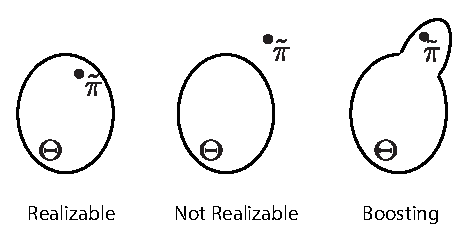
\includegraphics[width=0.5\textwidth]{f_figs/realizibility.eps}
\caption{
    \footnotesize
An illustration of the  of realizable. Denote a policy class $\Theta$ and a supervisor policy $\tilde{\pi}$, the supervisor's policy is realizable if it is contained in $\Theta$. We also illustrate Boosting, which can be thought of as attempting to grow the function class to achieve realizibility.}
\vspace*{-20pt}
\label{fig:teaserl}
\end{figure}

However, if the supervisor's policy is realizable on the states visited then performing  supervised learning is guaranteed to converge to the supervisor's policy as more training data is collected, which stems from a known property in statistics~\cite{anthony2009neural}. We show theoretically and empirically that active LfD methods can actually be harmful in this situation because they can train on states that the supervisor would never visit and thus lead to slower convergence. Furthermore, we theoretically show than when the supervisor is only realizable on states they are likely to visit, active LfD can actually not converge to the supervisor's policy.

We acknowledge though that in practice realizibility can be hard to achieve. Thus, we propose using boosting on the current robot's policy class to incrementally inflate the class size. Boosting works by growing a learner to correct its current mis-predictions. An interesting property of Boosting is that by incrementally growing the class size the bias-variance trade-off can scale in a much tamer way as opposed to a standard non-parameteric regressor~\cite{buhlmann2003boosting}. Thus, we can avoid over-fitting to the observed example from the supervisor. 

\mlnote{Still working on how to summarize all results}
Our contributions is showing, both theoretically and emprically that active LfD algorithms can achieve worse performance versus supervised LfD, if the function class is realizable. We also provide experiments on a physical robot setup with randomized human trials of teaching a robot how to singulate. 


\section{Related Work}
Below we summarize related work in active approaches in applications of Online LfD to robotics, sample complexity results and then work on reducing samples. \mlnote{Will update related work}


\noindent \textbf{Online LfD with an Expert Supervisor}
Online Learning from Demonstration in robotics has achieved numerous examples of completely model-free learning from high dimensional state representations, such as images. Successful robotic examples of Online Learning From Demonstration with an expert supervisor include applications to flying a quad-copter through a forest where the input is only image data taken from an on board sensor. 

Recently, Laskey et al. applied Online Learning from Demonstration to manipulation tasks such as surgical needle insertion \cite{laskeyshiv}, where a surgical robot correctly learns to insert a needle into tissue to prepare for suturing. Furthermore, Laskey et al. applied Online LfD to robotic de-cluttering, where a robot is given image data of a table with a variety of objects on it and must learn to push the obstacle objects aside to grasp a goal \cite{laskeyrobot}. 

Other succesful examples have been teaching a robotic wheel chair navigate to goal positions in the presence of obstacles and teaching a robot to follow verbal instructions to navigate across an office building \cite{kim2013maximum, duvallet2013imitation}. 

\noindent \textbf{Sample Complexity in Online LfD}
Sample complexity analysis in Online LfD is normally summarized as to results.  Ross et al. showed that a supervise learning approach (i.e. where no iterative online feedback is used) achieves an error rate that is quadratic in the time horizon, but is only an asymptotic bound \cite{ross2010efficient}. 

Ross et al. then models an iterative Online LfD algorithm known as DAgger as a Follow-The-Leader algorithms and gives regret bounds for strongly convex loss functions, however it also have linear dependence on $T$. We argue that both of these approaches can instead by thought of as traditional supervise learning, where the sample distribution is simply different than the distribution optimized over and model the problem as supervise learning with importance sampling weights. 

Finally of interest to us is the comparison to Reinforcement Learning methods. A common approach in RL for robotics is policy gradients, where a gradient is computed on the loss function based on sample estimates. Kakade et al. demonstrated that  a single gradient estimate can require on the order of cubic in the time horizon samples~\cite{kakade2003sample}. For perspective a robotic task has hundreds of time steps and can sometimes take minutes to sample a trajectory.

\noindent\textbf{Reducing Supervisor Burden in Online LfD} 
An interesting line of work in this field is applying active learning to the task of Online LfD, which has the promise to help reduce sample complexity. Active learning approaches to reducing supervisor burden only ask for supervision when the robot is uncertain about the
correct control to apply. Traditional active learning techniques like query-by-committee and uncertainty sampling have
been utilized for this purpose \cite{chernova2009interactive,judah2011active,grollman2007dogged}
Kim et al. demonstrated that due to the non-stationarity of the distribution of states encountered during
learning, the traditional active learning techniques may not be suitable.
Thus the use of novelty detection was proposed~\cite{kim2013maximum}. Laskey et al. introduced SHIV, using an active
learning approach tailored to high dimensional and non-stationarity state distributions and a modified version of the
One Class SVM classifier. This reduced the density estimation problem to a 
simpler regularized binary classification~\cite{laskeyshiv}. 


\section{Problem Statement}\label{sec:PS}
The goal of this work is to learn a policy that matches that of the supervisor's while asking the supervisor for as few examples as possible.

\begin{figure}
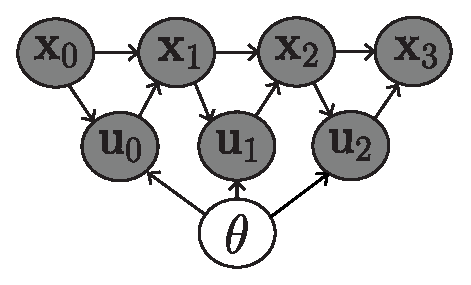
\includegraphics[width=0.5\textwidth]{f_figs/graph_model.eps}
\caption{
    \footnotesize
A graphical model of observed trajectory as a function of the hidden variable $\theta$.  We note that the dynamics and initial state distributions are dropped in this objective because they are conditionally independent of $\theta$, once the controls are observed. }
\vspace*{-20pt}
\label{fig:graphModel}
\end{figure}

\noindent\textbf{Modeling Choices and Assumptions}  We model the system dynamics as Markovian, stochastic, and stationary. Stationary dynamics occur when, given a state and a control, the probability of the next state does not change over time. 

We model the initial state as sampled from a distribution over the state space.
We assume a known state space and set of controls. We also assume access to a robot or simulator, such that we  can sample from the state sequences induced by a sequence of controls.   Lastly, we assume access to a supervisor who can, given a state, provide a control signal label. We additionally assume the supervisor can be noisy and imperfect, noting that the robot cannot surpass the level of performance of the supervisor. 

\noindent\textbf{Policies and State Densities.}
Following conventions from control theory, we denote by $\mathcal{X}$ the set consisting of observable states for a robot task, consisting, for example, of 
high-dimensional vectors corresponding to images from a camera, or robot joint angles and object poses in the environment.
We furthermore consider a set $\mathcal{U}$ of allowable control inputs for the robot, which can be discrete or
continuous. We model dynamics as Markovian, such that the probability of state $\mathbf{x_{t+1}}\in
\mathcal{X}$ can be determined from the previous state $\mathbf{x}_t\in\mathcal{X}$ and control input $\mathbf{u}_t\in
\mathcal{U}$: 
$$p(\bx_{t+1}|\bu_{t},\bx_{t}, \ldots, \bu_{0}, \bx_{0})=p(\bx_{t+1}|\bu_{t}, \bx_t)$$
We assume a probability density over initial states $p(\bx_0)$.
%We denote the probability density over the initial state also by $p:\mathcal{X}\to \mathbb{R}$. 

A trajectory $\hat{\tau}$ is a finite series of $T+1$ pairs of states visited and corresponding
control inputs at these states, $\hat{\tau} = (\mathbf{x}_0,\mathbf{u}_0, ...., \mathbf{x}_T,\mathbf{u}_T)$, where $\bx_t\in \mathcal{X}$
and $\bu_t\in \mathcal{U}$ for $t\in \{0, \ldots, T\}$ and some $T\in \mathbb{N}$.  
For a given trajectory $\hat{\tau}$ as above, we denote by ${\tau}$ the corresponding trajectory in state space,
${\tau} = (\bx_0,....,\bx_T)$.


A policy is a function $\pi: \mathcal{X} \to \mathcal{U}$ from states to control inputs. 
We consider a space of policies $\pi_{\theta}:\mathcal{X}\to \mathcal{U}$ parameterized by some $\theta\in \Theta$. Any such policy $\pi_{\theta}$ in an environment with probabilistic initial state density and Markovian dynamics
induces a density on trajectories of length $T+1$: $$p(\tau | \theta)=
p(\bx_0)\prod_{i=0}^{T-1}p(\bx_{t+1}|\bu_t,\bx_t)p(\bu_t|\pi_{\theta}(\bx_t))$$


A graphical model that demonstrates this relationship can be shown in Fig. \ref{fig:graphModel}. We note here that once the controls are observed in the graphical model the policy parameters are conditionally independent of the dynamics and probability of initial state distributions: $p(\bx_{t+1}|\bu_t,\bx_t)$ and $p(\bx_0)$. 


While we do not assume knowledge of the distributions corresponding to: $p(\bx_{t+1}|\bx_t,\bu_t)$, $p(\bx_0)$, $p(\bx_t|
\theta)$ or $p(\bx|\theta)$, we assume that we have a stochastic real robot or a simulator such that for any state
$\bx_t$ and control $\bu_t$, we can sample the $\bx_{t+1}$ from the density $p(\bx_{t+1}|\bu_t,\bx_t)$. 
Therefore, when 'rolling out' trajectories under a policy
$\pi_{\theta}$, we utilize the robot or a simulator to sample the resulting stochastic trajectories rather than
estimating $p(\bx|\theta)$ itself.


\noindent\textbf{Objective.} The objective of  policy learning is to find a policy that minimizes some known cost function $C(\hat{\tau}) = \sum^T_{t=1} c(\bx_t,\bu_t)$ of a trajectory $\hat{\tau}$. The cost $c:\mathcal{X}\times \mathcal{U}\to \mathbb{R}$ is typically user defined and task specific. 
For example, in the task of inserting a peg into a hole, a function on distance between the peg's current and desired final state is used \cite{levine2015end}.  

In our problem, we do not have access to the cost function itself. Instead, we only have access to 
a supervisor that can achieve a desired level of performance on the task. The supervisor provides the robot an initial set
an initial set of $N$ stochastic demonstration trajectories $\lbrace \tilde{\tau}^1,...,\tilde{\tau}^N \rbrace$. 
which are the result of the supervisor applying this policy. This induces a training data set $\mathcal{D}$ of all state-control input pairs from the demonstrated trajectories.

We are interesting in determining what parameter $\theta$ generates the sample demonstrations from the supervisors policy. The question can be framed as maximizing the conditional likelihood of the sample demonstrations conditioned on a given parameter $\theta$. 

$$\underset{\theta}{\mbox{max}} \prod^N_{n=1} p(\bx_0,n) \prod^T_{t=1} p(\bx_{t+1,n}|\bx_{t,n},\bu_{t,n})p(\bu_t|\bx_t,\theta)$$

In solving this optimization it is common to optimize the conditional log-likelihood, which maintains the same solution but breaks up the product terms into sums. 

$$\underset{\theta}{\mbox{max}} \sum^N_{n=1}\sum^T_{t=1}\mbox{log }p(\bu_t|\bx_t,\theta)$$

We note that the dynamics and initial state distributions are dropped in this objective because they are conditionally independent of $\theta$, once the controls are observed. 

The distribution $p(\bu|\pi_\theta(\bx))$ can be thought of a as modeling choice for the supervisor. One can assume in the continuous controls case that the supervisor is making decisions drawn from a uni-modal Gaussian distribution, which would yield the following objective:

\begin{equation}\label{eq:main_obj}
\hat{\theta} = \underset{\theta}{\mbox{argmax}} \sum^N_{n=1}\sum^T_{t=1}-|| \bu_{n,t} - \pi_{\theta} (\bx_{n,t})||^2_2.
\end{equation}

One could also model the supervise as making multi-modal decisions, such as when the supervisor encounters "fork in the road" situations, where either choice is acceptable. Traditionally  Eq. \ref{eq:main_obj}, has been known as the surrogate loss to denote a difference between the true cost function. We will refer the to function $l : \mathcal{U} \times \mathcal{U} \rightarrow \mathbb{R}$ as the surrogate loss through out this paper. The surrogate loss can either be an indicator function as in classification or a continuous measure as indicated above.  This rewrites the objective as follows: 

\begin{equation}\label{eq:main_obj}
\hat{\theta} = \underset{\theta}{\mbox{argmin}} \sum^N_{n=1}\sum^T_{t=1} l(\bu_{n,t}, \pi_{\theta} (\bx_{n,t})).
\end{equation}


 The above objective can be challenge to solve because the supervisors policy, $\tilde{\pi}$ may not be realizable in the space $\Theta$, or functions that represent the robot's policy, or it may be contained but not able to be found do to local optimization methods, such a gradient descent for neural networks.  Thus leading to a mismeasure in the distribution trained on and tested on. 
 
 Prior work ~\cite{ross2010reduction}  proposed an iterative method that solves this problem by aggregating data to converge to a distribution induced by the robot's policy. We review this approach in Sec. \ref{sec:DAgger}.
 




\section{DAgger}\label{sec:DAgger}
Ideally the solution for Eq. \ref{eq:main_obj}, $\hat{\theta}$ would be a sample estimate of $\tilde{\pi}$. However if $\tilde{\pi} \nsubseteq \Theta$ or is not realizable, then one approach is to try and agree with supervisor on the distribution induced by the robot's policy $p(\tau|\hat{\theta})$ because those are the states the robot is most likely to visit. 

A challenge occurs though when trying to fit a function that agrees with the supervisor on the distribution of states induced by the policy. The problem stems from not knowing what the distribution will be after the policy is optimized. To tackle this problem an iterative algorithm was proposed that under certain conditions converges to optimizing on the distribution induced by the policy. 


 \subsection{Algorithm}
Instead of  minimizing the surrogate loss, in Eq. \ref{eq:main_obj},  DAgger attempts to find the distribution the final policy will end up on. In the not realizible situation, this can help reduce surrogate loss. 
DAgger~\cite{ross2010reduction} attempts this by iterating two steps: 1)
computing the policy parameter $\theta$ using the training data $\mathcal{D}$ thus far, and 2) by executing the policy
induced by the current $\theta$, and asking for labels for the encountered states. 
 
\subsubsection{Step 1}
The first step of any iteration $k$ is to compute a $\theta_k$ that minimizes surrogate loss on the current dataset $\mathcal{D}_k=\{(x_i,u_i)|i\in\{1,\ldots,M\}\}$ of demonstrated state-control pairs (initially just the set $\mathcal{D}$ of initial trajectory demonstrations):

 \vspace{-1ex}
\begin{align}\label{eq:super_objj}
\theta_{k} = \underset{\theta}{\argmin} \: \sum_{i=1}^{M} \sum_{t=1}^T  l(\pi_{\theta}(\bx_{i,t}),\bu_{i,t}).
\end{align}

This can be observed as minimizing the empirical risk on the aggregate dataset of all examples seen so far, note that equal weight is giving to each example regardless of high likely they under the current policy~\cite{scholkopf2002learning}. 
 

 \subsubsection{Step 2}
The second step at iteration $k$, DAgger rolls out the current policy, $\pi_{\theta_{k}}$, to sample states that are likely under $p(\tau|\theta_{k})$.  For every state visited, DAgger requests the supervisor to provide the appropriate control/label. Formally, for a given sampled trajectory  $\hat{\tau} = (\bx_0,\bu_0,...,\bx_T,\bu_T )$, the supervisor provides labels $\tilde{\bu}_t$, where $\tilde{\bu}_t \sim \tilde{\pi}(\bx_t) + \epsilon$, where $\epsilon$ is a  zero mean noise term, for $t\in \{0, \ldots, T\}$.
The states and labeled controls are then aggregated into the next data set of demonstrations $\mathcal{D}_{k+1}$:
$$D_{k+1}=\mathcal{D}_k \cup \{(\bx_t,\tilde{\bu_t})|t\in\{0,\ldots,T\}\} $$

Steps 1 and 2 are repeated for $K$ iterations or until the robot has achieved sufficient performance on the
task\footnote{In the original DAgger the policy rollout was stochastically mixed with the supervisor, thus with
    probability $\beta$ it would either take the supervisor's action or the robots. The use of this stochastically mix
    policy was for theoretical analysis and in practice, it was recommended to set $\beta = 0$ to avoid biasing the
sampling~\cite{NIPS2014_5421,ross2010reduction}}.

\subsection{Interpretation of DAgger}
As DAgger iterates between optimizing the policy and gathering data, it trains an estimator on the distribution defined as $\frac{1}{K} \sum^K_{k=1} p(\tau|\theta_k)$. Since the goal of DAgger is to train the robot's policy on the distribution induced by the current policy $p(\tau|\theta_k)$, it is interesting to think under what conditions is the following true: 

$$\frac{1}{K} \sum^K_{k=1} p(\tau|\theta_k) = p(\tau|\theta_K)$$

It can be shown that when $$||\theta_k - \theta_{k+1} ||_{\infty} \leq \epsilon$$ and $\epsilon \rightarrow 0$ as $K \rightarrow \infty$ the above statement would be true due to the properties of expectation. This property of convergence to the final distribution is illustrated in Fig. \ref{sec:DAgger}. 

\begin{figure}
\centering
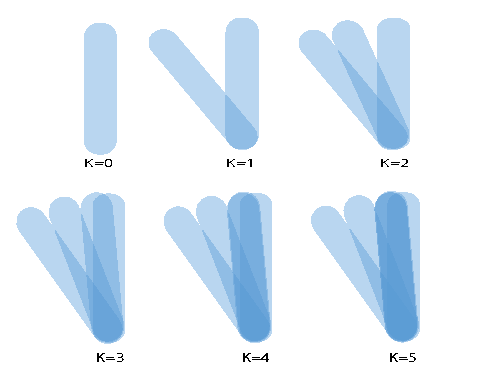
\includegraphics{f_figs/dagger.eps}
\caption{
    \footnotesize
An illustration of the evolution in distributions when running DAgger. In iteration $K=0$, the dataset is just the supervisor's demonstrations. The through iteratively rolling out the policy the density over the data can converge to the distribution induced by the policy at $K=5$. The darker regions correspond to an area of higher density. [PLANNING ON UPDATING FIGURE]}
\vspace*{-20pt}
\label{fig:graphModel}
\end{figure}

Under these conditions DAgger is able to sample and train on the states the robot is likely to see. This can allow one to improve the performance of the robot's policy despite not being able to perfectly match the supervisor's policy. However this method can have several limitations 1) it can require more data than necessary because a large number of the states the supervisor labels will have low probability at the end of learning 2) it can be hard for a human to retro-actively provide feedback since they have to predict how the dynamics would behave under their proposed control. 

In light of these limitations, we are interested in overcoming the model mismatch between the robot's policy and the supervisors. By iteratively weighting states that are hard to predict and growing the model to accommodate them. This technique is known as boosting, which we define in the next section. 



\section{Supervised LfD}
While DAgger handles the problem of model mismatch via optimizing on the distribution induced by the robot, we will instead assume realizability is achievable and leverage supervise LfD.  

\subsection{Supervised LfD}
In supervised LfD, $M$ demonstrations are collected from the supervisor's distribution $p(\tau|\tilde{\pi})$ and the following objective is minimized: 

$$\underset{\theta}{\mbox{min}} \: \frac{1}{M} \sum^M_{m=1} \sum^T_{t=1} l(\pi_{\theta}(\bx_{t,m}), \tilde{\pi}(\bx_{t,m}))$$

This is known as empirical risk minimization and in Sec. \ref{Sec:theory}, we show that this converges to the supervisor's policy if it is realizable. 

If the supervisor's policy is not realizable though than pure supervised learning could suffer in performance from not being active. Thus, we propose using Boosting to help inflate our model class to achieve realizability for observed demonstrations from the supervisor. 

\subsection{Boosting for Machine Learning}
The idea of boosting is to search for a robot's policy that lies not in the space of $\Theta$, but of $\mbox{lin}(\Theta)$ or linear combinations of the functional space. Boosting can be thought of searching for a function class that best matches the supervisor, but does not overly increase complexity~\cite{buhlmann2003boosting}.

Boosting operates by examining the error, or misclassifications, in the current training set at each iteration, $k$. Then weights the points higher that are misclassified using a specified function $f$ and learns a new $\pi_{\theta_k}$ parameter on this distribution.  Then the robot policy is updated as $\pi_{\sum \theta} = \sum^K_{k=1} w_k \pi_{\theta_k}$, where the policy is now an ensemble of weaker policy representations. An outline of the algorithm can be shown in Algorithm 1.

It has been shown that this process can be interpreted as performing gradient descent for a policy representation in the space of $\mbox{lin}(\Theta)$ and in the case of convex loss functions convergence to the best policy in this class is obtainable~\cite{mason1999boosting}.

\begin{algorithm}\label{alg:boosting}
$D_n = 0$ \;
 \For{k = 0,...,K}{
  Learner chooses \; 
   $\theta_k = \underset{\theta}{\mbox{argmax}}  \sum^N_{n=1} D_n  \times  l(\pi_{\theta}(\bx_n),\tilde{\pi}(\bx_n))$\;
Choose $w_{k+1}$\; 
Let $\pi_{\sum \theta} = \sum^k_{k=0} w_k \pi_{\theta_k}(\bx) + w_k \pi_{\theta_k}(\bx)$\;
$D_n = f(l(\pi_{\sum \theta}(\bx_n),\tilde{\pi}(\bx_n)))$
 }
 \caption{Boosting}

 
 
\end{algorithm}



\section{Theoretical Analysis} \label{Sec:theory}
In this section, we are interesting in analyzing supervised LfD and active LfD when the supervisor $\tilde{\pi}$ is realizable, or $\tilde{\pi} \in \Theta$.  We first analyze the situation where the supervisor is realizable in all of the workspace and show convergence for supervised LfD and active LfD to $\tilde{\pi}$. Then we look at the case where the supervisor is only realizable in places they are likely to visit and show that only supervised LfD is guaranteed convergence.

We assume throughout this section a bounded surrogate loss in the range of $[0,1]$ and that during minimization of the expected risk, the best function in the function class can be found. Examples of when these assumptions can be satisfied is if your robot has bounded controls and you are using a convex policy class, such as kernelized regression. 

\subsection{Realizable Everywhere}
Since we know that $\tilde{\pi} \in \Theta$ and that we can find the best fit for $\tilde{\pi}$ given the observed examples. Then the only reason that $\hat{\theta} \neq \tilde{\pi}$ is because not enough examples from the supervisor have been collected. 

Understanding how much data is needed to learn a function, is a well studied problem known as sample complexity analysis~\cite{anthony2009neural}. In this literature they use different metrics to describe the complexity of a function class and show rates on which a given function class would converge to the real solution. We refer the reader to \cite{anthony2009neural}, for a review of such topics. 

A main result from this literature is that under the conditions we have described the following statement is true: \\

\begin{theorem}\label{thm:sup}
For a policy, $\hat{\theta}$ found via Supervised LfD, from $m$ trajectories collected from the supervisor the following is true with probability at least $1- 2\mbox{exp} (-m\delta^2/8)$

$$E_{p(\tau|\tilde{\pi})} l(\pi_{\hat{\theta}}, \tilde{\pi}) \leq 2R_{\Theta}(m) + \delta+ O(\frac{1}{\sqrt{m}})$$\\

\end{theorem}

In this result, $R_{\Theta}$ corresponds to the Rademacher complexity of the given function class $\Theta$. The Rademacher complexity is a measure of much a function can fit to random noise, more complex function classes can fit better and thus leading to slower rates of convergence. 

The key take away from from this theorem  is that at a non-asymptotic rate of demonstrations the surrogate loss will be zero on the distribution of the supervisor, thus corresponding to exact agreement between robot and supervisor. The exact rate itself will vary as a function of Rademacher Complexity of $\Theta$. 

In active LfD, instead of collecting all $m$ demonstrations as samples from $p(\tau |\tilde{\pi})$, at each $k$ iteration  samples are taken from the current policy distribution $p(\tau|\hat{\theta}_k)$.  

Since, we assume the supervisor's policy is realizable in all parts of the workspace, then we can still determine $\tilde{\pi}$ from this sampled data. However, because we previously showed that the $\hat{\theta}$ will converge to $\tilde{\pi}$, then sampling from a distribution that isn't $p(\tau|\tilde{\pi})$ could result in querying the supervisor for demonstrations that are not informative. \mlnote{writing a formal proof for this, will update} Thus, resulting in a potentially slower convergence. We demonstrate this effect experimentally in Sec. \ref{sec:gdw}. 

\subsection{Realizable only on Supervisor's Support}
Consider the situation, where the supervisor is only realizable on the places they are likely to visit, or within the support of $p(\tau|\tilde{\pi})$. 

For instance if a supervisor trying to teach the task of driving down a highway, then they will stay within the lanes of the road and have a relatively smooth policy of going forward at a constant speed. However, if the supervisor is forced to veer off the road their resulting policy will become a much more complex maneuver to avoid crashing. 

While supervised LfD never forces the supervisor to visit these states, active LfD  could learn a  policy that includes data from these more complex regions. Thus, potentially preventing active Lfd from ever converging to the true supervisor. Denote $\hat{\theta}_S$ as the policy found by supervisor LfD and $\hat{\theta}_a$ as that found by active LfD and $m$ the number of demonstrations. \\

\begin{theorem}
If $\tilde{\pi} \in \Theta$ only on the support of $p(\tau|\tilde{\pi})$ and $m\rightarrow \infty$, then $\hat{\theta}_S \rightarrow \tilde{\pi}$ but there exists situations where $\hat{\theta}_A$ does not converge to $\tilde{\pi}$.\\
\end{theorem}

\begin{proof}
In order to prove the first part of the statement, that $\hat{\theta}_S \rightarrow \tilde{\pi}$ as  $m \rightarrow \infty$. We  use the result of Theorem 1 and note that all training data colected is in the region of realizibility.\\ 

In the second part of the theorem, convergence of active LfD techniques are not guaranteed because they could end up sampling part of the state space outside of the support of $p(\tau|\tilde{\pi})$.

This can happen if there exists an iteration $k \in 1:K$ where $p(\tau | \hat{\theta}_k)$ exhibits non-zero measure outside the support of $p(\tau |\tilde{\pi})$. Thus, collecting training data in parts of the state space where the policy is not realizable, which can result in the solution to the empirical risk minimization not finding the supervisor's policy because it has to cope with model error. 

\end{proof}

While in practice this problem can be potentially overcome by increasing the complexity of $\Theta$, to make the supervisor realizable everywhere. It would result in a large Rademacher complexity and subsequently more training data. Thus, if the supervisor is less complex on their own distribution using supervised LfD can save data. 


\section{Experiments}


\begin{figure*}
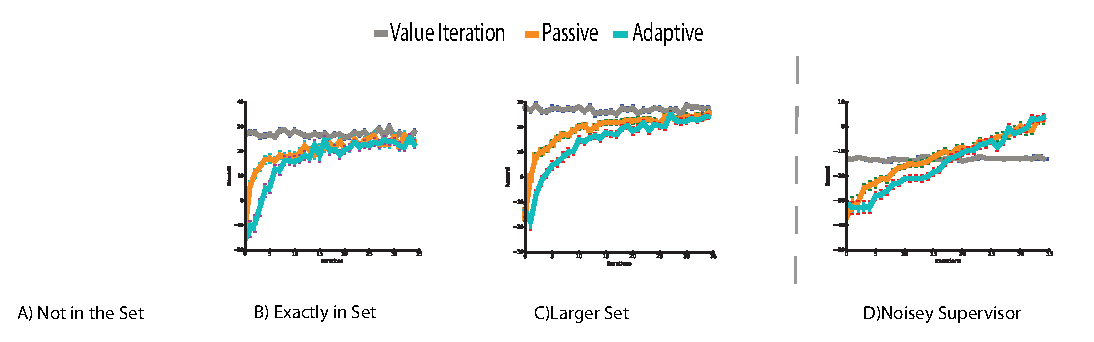
\includegraphics{f_figs/var_grid.eps}
\caption{
    \footnotesize
Shown above is the expected reward obtained for Value Iteration, which is the optimal supervisor, Supervise learning using Adaboost, DAgger and Supervise learning. All results are averaged over 1500 trials. In A) we demonstrate the four approaches for a given dynamics and initial state distributions, Adaboost converges fastest to the supervisor. In B), we double the noise in the dynamics, which causes the robot to cover a lot more states. Adaboost is still able to achieve faster convergence, which suggests DAgger does not help in producing a covering of states. Finally, in C) we increase the initial state variance by 5x, to try and see if over-fitting to a small sample size is possible. Results suggests that the effects of over-fitting persists in both DAgger and Adaboost.}
\vspace*{-20pt}
\label{fig:var}
\end{figure*}

We provide experiments in a simulated GridWorld environment, which allows for us to vary noise in the dynamics and initial state distribution: $p(\bx_t|\bx_t,\bu_t)$ and $p(\bx_0)$, with a deterministic supervisor. Then we  train a Zymark robot to singulate objects from each other, which allows for us to look at high dimensional image environments and work with a human supervisor. 
\subsection{GridWorld}\label{sec:gdw}
In a simulated GridWorld, we have a point robot that is trying to reach a goal state, at which it receives $+10$ reward. The robot receives $-10$ reward if it touches a red state, as shown in Fig. \ref{fig:grid_world}. The robot has a state space of $(x,y)$ coordinates and a set of actions consisting of $\lbrace$LEFT,RIGHT,FORWARD,BACKWARD,NONE$\rbrace$, where NONE indicates staying at the current stop. For the transition dynamics $p(\bx_{t+1}|\bx_{t},\bu_t)$, the robot goes to an adjacent state that does not correspond to the intended control with probability $0.2$. 

We use Value Iteration to compute an optimal supervisor for our grid world domain. The optimal policy must learn to be robust to the noise in the dynamics, reach the goal state and then stay there. The robot policy is represented as a decision tree with a maximum depth of $3$ and is trained using Sci-Kit Learn~\cite{scikit-learn}. We used a fix time horizon of $T=40$, which gives the robot enough time to get to the goal state. 


\noindent \textbf{Realizable vs. Not Realizable} In Fig. \ref{fig:low_var}, we show supervise learning with the fixed decision tree, DAgger and supervise learning with boosting applied to the decision tree. Similar to prior work supervise learning with a fixed decision tree does worse than DAgger, which iteratively determines the distribution it policy induces and minimize the expected risk on it. However, DAgger is outperformed by the boosted learner, which is able to match the supervisor's controls during train and induce the same distribution. 

To see how the results change when the variance is increased in the graphical model, we double the dynamics noise. Now, $p(\bx_{t+1}|\bx_t,\bu_t)$ causes the robot to go an adjacent state that does not correspond to the intended control with probability $0.4$. In Fig. \ref{fig:high_var}, we show that despite the large variance the relative results of DAgger, Boosted Supervised and Supervised remains the same. However, more data is still need to learn the policy, which corresponds to an increase in variance in the sampled distribution. We also note that Value Iteration optimal supervisor does much worse due to instability in control. 

\begin{figure}
\centering
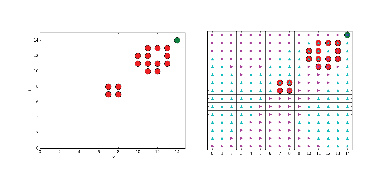
\includegraphics{f_figs/grid_world.eps}
\caption{
    \footnotesize
Left: An example of the grid world domain, where the robot must reach the goal (green) state and avoid the red objects, for which it receives negative reward. The dynamics in this enviroment are stochastic, which requires a robot to learn a control policy that is robust to variance. Right: Is the optimal policy with respect to the expected discounted reward computed by our supervisor, Value Iteration.  }
\vspace*{-10pt}
\label{fig:grid_world}
\end{figure}

\noindent \textbf{Realizable Everywhere} 
We are next interested in the situation when both DAgger and Supervised Learning are realizable. We use a 3D gridworld in this test domain that includes the additional action of UP and DOWN. We do this because to observe the effects of sub-optimally sampling data its important to create a larger workspace. 

In Fig. \ref{fig:r_eq}, we show Boosted DAgger against Boosted Supervisor in two situation one with low initial state variance and one with higher initial state variance. The low initial state variance shows Boosted DAgger performing similar to Boosted Supervisor, however as the initial state variance is increased the robot's policy makes more mistakes and collects demonstrations in states the supervisor is unlikely to visit. 


\begin{figure}
\centering
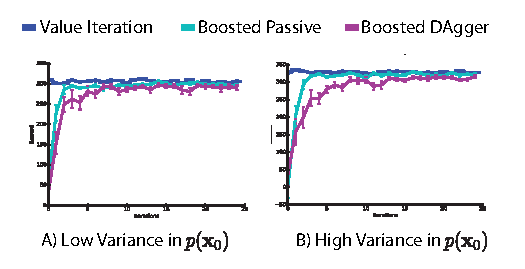
\includegraphics{f_figs/r_ev.eps}
\caption{
    \footnotesize
Shown is Boosted Supervisor compared against Boosted DAgger in a 3D gridworld domain with each iteration corresponding to a demonstration given via the supervisor controlling the system or retro-actively, respectively. All results are averaged over 1000 trails. With low initial state variance the performance is similar, however as the initial state variance is increase DAgger queries the supervisor for less informative demonstrations. Thus, resulting in slower convergence.   }
\vspace*{-20pt}
\label{fig:r_eq}
\end{figure}



\noindent \textbf{Realizable only on Supervisor's Support} 


\subsection{Planar Singulation}




  



\section{Conclusion}
\mlnote{This is specific to the theoretical analysis section}
In conclusion, we have shown that by knowing what distribution the robot is likely to encounter we can achieve more representative bounds on the performance of our policy. 

By achieving the familiar bound of Rademacher Complexity, we can now apply techniques such as Metric Entropy, Fat Shattering and VC Dimension to achieve sample complexity terms for both convex class and non-convex, which can be more enlightening than the previous FTL analysis. 

However, the bounds show a strong dependence on how large the importance sampling weights can become. This implies that if our policy starts to deviate from the training set during its empirical risk minimization. It is likely that the effective sample size could be quite low and thus require more samples. We present several ways to control for this factor and will begin experimentally seeing the effects.  

\bibliographystyle{IEEEtranS}
\bibliography{references}


\end{document}